\newpage
\subsection{Création des rayons projetés}
\subsubsection{Création d'une base orthonormée pour la caméra}
Pour projeter les rayons vers la scene 3D, on va d'abord avoir besoin de donner une direction à chacuns de ces rayons. Pour cela, il va nous falloir une base orthonormée de vecteurs pour définir le plan de l'écran.
\\
\\ 
On suppose que l'on connait $tilt$ et $pan$ qui sont les angles de la caméra donnés par le curseur. 
\begin{align*}
    e_z =&  (cos(tilt)\times sin(pan) ,\ sin(tilt) ,\ cos(tilt)\times cos(pan))\\
    e_x =&  normalize(e_z \wedge (0,1,0) )\\
    e_y =& e_x \wedge e_z\\
\end{align*}

Avec $normalize(\cdot ) = \frac{\cdot }{\| \cdot  \|}$\\ \\  
Ainsi, on a $e_x$ et $e_y$ qui forment le plan de l'écran, et $e_z$ qui est dans le sens opposé de la direction de la caméra.\\ \\ 
\textbf{Remarque} : Cette base de vecteurs est orthonormée.

\subsubsection{Création des vecteurs directeur pour chaque pixel}
Pour chaque pixel de l'écran, on va associer un vecteur directeur. Ce vecteur est calculé avec $x$ et $y$ les coordonées du pixel et FL la longueur focale $(x,y,FL\in \mathbb{R})$: 
\begin{align*}
    Direction &= normalize(x\times e_x + y\times e_y - FL\times e_z)\\
\end{align*}

On obtient ainsi un vecteur directeur pour chaque pixel de l'écran.
\begin{figure}[h]
    \centering
    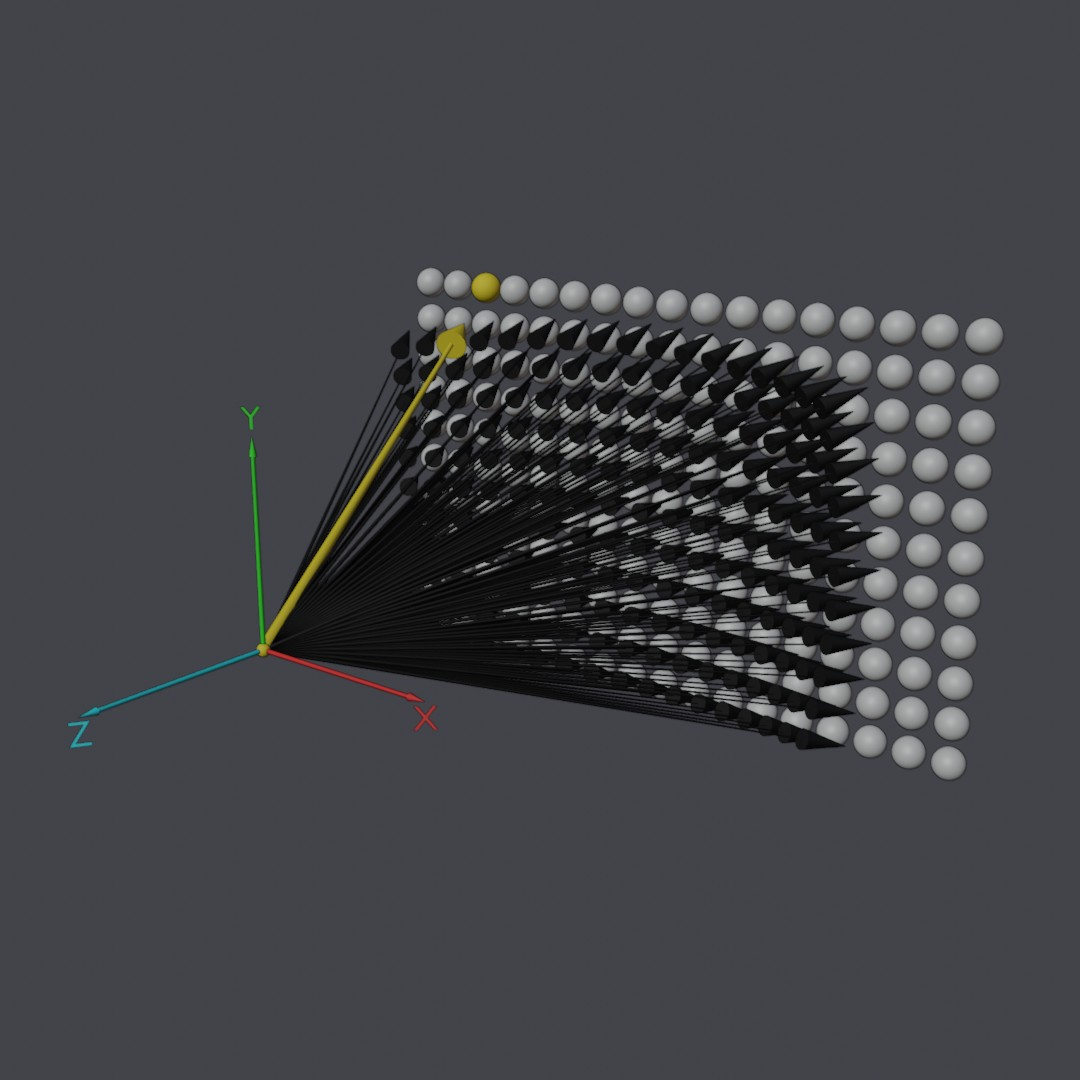
\includegraphics[width=7cm]{images/vectorscreen1.jpg}
    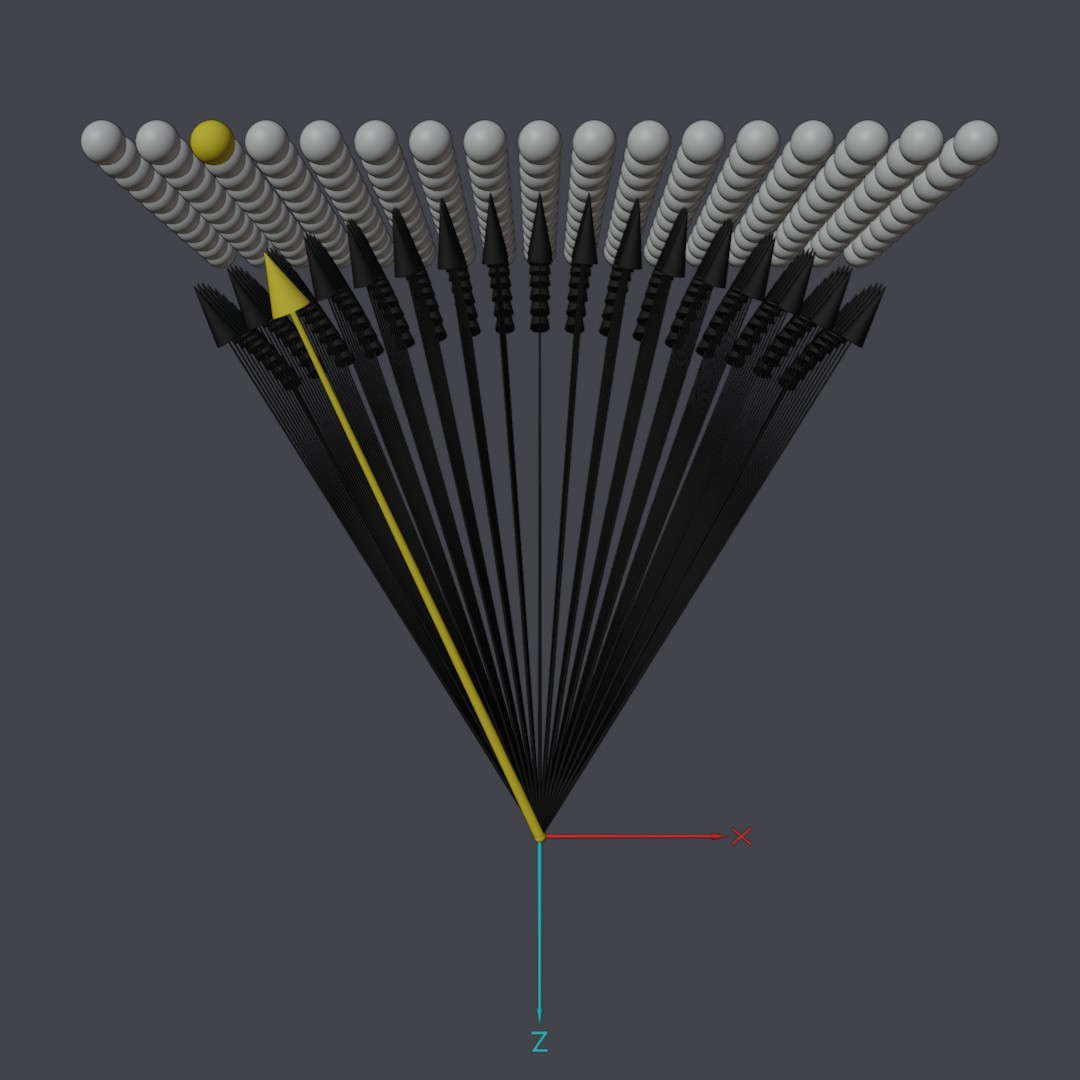
\includegraphics[width=7cm]{images/vectorscreen2.jpg}
    \caption{Visualisation des vecteurs associés aux pixels de l'écran, chaque sphère représentant un pixel }
    \label{fig:screenvectors}
\end{figure}